\chapter{Numerical Needle Probe Approach}
\label{sec:numerical-np}
\bigskip

\section{Introduction} 
\label{sec:numerical-np:introduction}

Numerical experiments simulated needle probes in anisotropic mediums with
three-dimensional finite element heat transfer models in COMSOL 3.5a. While the
models themselves were relatively simple, attempting to automate a parameter
study in COMSOL 3.5a with respect to the anisotropic material properties proves
difficult.

\section{Geometry and Domain Properties}

\begin{figure}[h]
\centering
\includegraphics[width=0.8\textwidth]{fig/domain_2.png}
\caption{A COMSOL screenshot showing the geometry of the finite element model, which consists of a metal needle in a sphere of a snow-like material.}
\label{fig:domain}
\end{figure}


\begin{table}[h]
\centering
\caption{Constants Used in Numerical Models}
\begin{tabular}{r | l}
radius of needle & \(0.25\) mm\\
length of needle & \(10\) cm\\
radius of snow & \(40\) cm\\
\hline
density of needle & \(8000\) kg/\(\textrm{m}^3\)\\
\(C_P\) of needle & \(460\) \(\flatfrac{\textrm{J}}{\textrm{kg}\cdot\textrm{K}}\) \\
\(q\) of needle & \(0.5\) W/m\\
\(k\) of needle & \(160\) W/m\(\cdot\)K\\
\hline
density of snow & \(200\) kg/\(\textrm{m}^3\)\\
\(C_P\) of snow & \(2050\)  \(\flatfrac{\textrm{J}}{\textrm{kg}\cdot\textrm{K}}\)
\end{tabular}
\label{tab:constants}
\end{table}

The needle is simulated as a long, thin steel cylinder embedded in the center
of a sphere of a snow-like material (called snow in this model), as in figure \ref{fig:domain}. While most of the dimensions
and material properties are held constant (see Table \ref{tab:constants}), the
anisotropic conductivity of the snow is parameterized in the form
of a  \(3\times3\) symmetric, positive definite matrix.  In practice, this is
done by specifying a diagonal matrix \(\Lambda\) with positive eigenvalues
\(k_{xy}\) and \(k_z\) and a rotation matrix \(R\) around the \(x\) axis, and
then defining \(K = R^T\Lambda R\) as in Equation \ref{eq:rotdiagrot} :

\begin{equation}
\label{eq:rotdiagrot}
K = \begin{bmatrix}
\cos(\theta) & 0 & \sin(\theta)\\
0 & 1 & 0\\
-\sin(\theta) & 0 &\cos(\theta)
\end{bmatrix}
\begin{bmatrix}
k_{xy} & 0 & 0\\
0 & k_{xy} & 0\\
0 & 0 & k_z
\end{bmatrix}
\begin{bmatrix}
\cos(\theta) & 0 & -\sin(\theta)\\
0 & 1 & 0\\
\sin(\theta) & 0 &\cos(\theta)
\end{bmatrix}
\end{equation}

The boundary conditions on the surface of the sphere enforce zero heat flux,
and the radius of the sphere is chosen such that the sphere approximates an
infinite medium.

Point temperatures recorded are the center of the needle, which corresponds to
the location of the thermocouple used in real-world experiments, and six points
on the surface of the snow, to ensure that the sphere is sufficiently large by
checking for a near-zero increase in temperatures on these points. In these
models, the increase in temperature is on the order of \(10^{-14}\) degrees
Kelvin.

\section{MATLAB in Geometry-Based Parameter Studies Using COMSOL 3.5a}
\label{sec:numerical-np:matlab}

Unfortunately, COMSOL 3.5a does not have the facilities necessary to implement a
geometry-changing multi-parameter study as required from the GUI alone. However,
COMSOL 3.5a does have facilities for scripting with MATLAB.

MATLAB code written to implement the parameter study was largely auto-generated
by COMSOL, by building a base model in COMSOL 3.5a and exporting to an m-file.
This code is split into two parts: The meshing code, and the solving code.
These pieces of code are wrapped in functions, called ``mesher'' and ``solver''
respectively, and used by a main procedure called ``worker.m.'' Contained in
``worker.m'' is a MATLAB structure with the constants outlined in section
\ref{sec:numerical-np:domain} called ``params''. The structure also contains a
list of angles yet to be solved for, and the times for which to solve.

The meshing function is called ``mesher'' and takes an angle
(in degrees) and the params structure as arguments, and is for the most part
simply code generated by COMSOL:

%% MESHER %%%%%%%%%%%%%%%%%%%%%%%%%%%%%%%%%%%%%
\small
\begin{minted}{matlab}
function fem=mesher(angle,params)
    % mesh_generate(angle)
    % generates a mesh for the given angle. 

    fprintf(['meshing for angle=' num2str(angle) '...\n']);

    flclear fem

    % Hand-modified COMSOL-generated code here
\end{minted}
\normalsize

The COMSOL code was changed to use the arguments passed to ``mesher'' instead of
the values used in the original model. For example:

\small
\begin{minted}{matlab}
    % Geometry
    g1=sphere3( num2str(params.rsnow), ...
                'pos', {'0','0','0'}, ...
                'axis', {'0','0','1'}, ...
                'rot','0');
    g2=cylinder3( num2str(params.rneedle), ...
                  num2str(params.lneedle), ...
                  'pos', {num2str(-params.lneedle/2),'0','0'}, ...
                  'axis', {'1','0','0'}, ...
                  'rot','0');
\end{minted}
\normalsize

Notice that, in this code, ``theta'' is never actually used. This is
because, in early iterations of the code, the needle was rotated by the angle
``theta.'' However, this caused unpredictable errors from COMSOL's meshing
procedures, so the anisotropic thermal properties of the snow are changed
instead, as outlined in section \ref{sec:numerical-np:domain}. However, the
argument is retained in order to avoid editing other legacy code in the model.

Afterwards, geometry is labelled and a mesh is initialized and refined using
code generated by COMSOL, and returns the COMSOL ``fem'' structure.

\small
\begin{minted}{matlab}
    % Hand-modified COMSOL-generated code here
    fem=multiphysics(fem);
end
\end{minted}
\normalsize

This ``fem'' structure may then be passed to the ``solver'' function, along
with parameters describing the snow's material properties and the needle's
orientation with respect to the snow. Similarly, the ``solver'' function is
mostly COMSOL code wrapped in a function. It is in this block that parameters
and the material properties are attached to the domain:

\small
\begin{minted}{matlab}
    % densities
    equ.rho = {params.density_snow,params.density_needle};
    equ.init = 0;
    equ.shape = 2;
    % Heat capacities
    equ.C = {params.cp_snow,params.cp_needle};
    % Wattage
    equ.Q = {0,params.q_needle/pi/(params.rneedle)^2};
    % Heat conductivities
    arr = [ cos(theta*pi/180), 0, sin(theta*pi/180); ...
            0, 1, 0; ...
            -sin(theta*pi/180), 0, cos(theta*pi/180) ]; %rotation matrix
    equ.k = { symmetric_tocell(arr*diag([kxy,kxy,kz])*(arr')), ...
              params.k_needle };
\end{minted}
\normalsize

This is also where the symmetric matrix is generated, as described in section
\ref{sec:numerical-np:domain}. ``symmetric\_tocell'' is a helper function which
converts symmetric matrices of the form \\
\texttt{[a1 a2 a4; a2 a3 a5; a4 a5 a6]} to the form \texttt{\{a1, a2, a3, a4, a5, a6 \}}.

Code to plot the solution has been replaced with code that saves the
temperature data at the center of the needle, and the average temperature of the
six points at the surface of the sphere, to MATLAB variables:

\small
\begin{minted}{matlab}
    % Integrate
    T_thermistor=postint(fem,'T', ...
               'unit','K', ...
               'recover','off', ...
               'dl',8, ...
               'edim',0, ...
               'solnum','all');

    % Integrate
    T_surf_avg=postint(fem,'T', ...
               'unit','', ...
               'recover','off', ...
               'dl',[1,2,3,4,10,11,12,13], ...
               'edim',2, ...
               'solnum','end');
\end{minted}
\normalsize

Finally, the data is packed into a cell array, and the ``angles'' parameter
is updated:

\small
\begin{minted}{matlab}

    answer={[fem.sol.tlist; T_thermistor],T_surf_avg};
    angles = params.angles(2:length(params.angles));

    %{
    flsave([ 'fem-' num2str(theta) '-' ...
             num2str(kxy) '-' num2str(kz) ...
             '.mph']);
    }%

    save('angles.m', 'angles');
end
\end{minted}
\normalsize

In some runs, the fem structure was exported back to the COMSOL format for
further study, such as viewing the temperature distribution over the entire
domain as in figure \ref{fig:comsol}.

\begin{figure}[h]
\centering
\includegraphics[width=0.6\textwidth]{fig/35892_elem_1097s.png}
\label{fig:comsol}
\caption{A side-view of COMSOL's results, focusing on the needle. Colors indicate temperature.}
\end{figure}

\section{Automatic Calculation of Conductivity from Simulated Time/Temperature Data}

Results from COMSOL are automatically fitted against the linear model with
respect to \(\ln(t)\) by ``dropping'' early \((t,T)\) datapoints until the
correlation coefficient of the remaining points was sufficiently high, as in Figure \ref{fig:curvefit}. Then, a
linear curvefit is applied to these remaining points. Finally, the slope of this fit is
used to calculate \(k_{\textrm{meas}}\).

\begin{figure}[h]
\centering
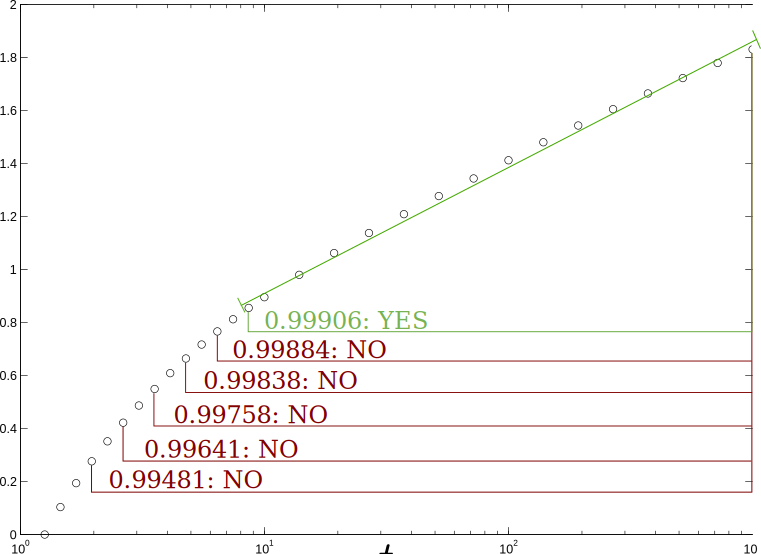
\includegraphics[width=0.6\textwidth]{fig/curvefit.png}
\caption{An illustration of the method used to find the "long-time" slope of the numerical simulations, which used a correlation coefficient to estimate the "straightness" of a section.}
\label{fig:curvefit}
\end{figure}

\section{Calculation and Serialization of Results}

These functions are called by ``worker.m,'' which is used to run multiple
tests and save the results:

%% WORKER %%%%%%%%%%%%%%%%%%%%%%%%%%%%%%%%%%%%%
\small
\begin{minted}{matlab}
function worker(kxy,kz)
    load('angles.mat', 'angles');
    angles
    [kxy,kz] = meshgrid(kxy,kz);
\end{minted}
\normalsize

Here, we can see ``worker.m'' loading a list of angles from an ``angles.mat''
file, which is MATLAB's native serialization format. This is because this particular install of COMSOL 3.5a
tends to have segmentation faults with relative regularity. So, a
solution was written where angles are serialized such that the
process can continue on the last unfinished angle. Unfortunately, because the
process hasn't been written to recover previously-solved conductivities at that
angle, the process can only handle a small subset of conductivity combinations
during a given run. The general method for iterating through all the different
test combinations is laid out here:

\small
\begin{minted}{matlab}
    mesh = mesher(0,params);
    for angle=angles,
        try
            solutions = arrayfun(@(x,y) solver(x,y,mesh,angle,params), ...
                            kxy,kz, 'UniformOutput', false);

            % . . .

            solutions = {cellfun(@(tsd) {fitter(tsd{1}(1,:),tsd{1}(2,:), ...
                                             0.999,params), ...
                             tsd{1}, tsd{2}}, ...
                         solutions, 'UniformOutput', false)};

            % . . .

        catch exception
            % Handles exceptions here
        end

\end{minted}
\normalsize

The reason that this code can't recover solved conductivity combinations
after a segmentation fault is because of the use of ``arrayfun,'' which acts 
similarly to the ``map()'' functions seen in other languages, such as perl and
python. Mapping functions return an array of the same size of the input but with the
corresponding results of the function applied to it. For example,
\texttt{map(lambda x: 2*x, [1, 2, 3])} will return \texttt{[2, 4, 6]} in python.

As a result of these manipulations, the results are organized into a nested
cell array which mirrors the format of the two MATLAB matrices k\_xy and k\_z,
as reflected in the use of ``arrayfun.'' The data in each slot of the
nested array is itself a cell array containing the simulation results, organized as shown
in Figure \ref{fig:cellarray}.

This section of code also has exception handling, as there are often issues when
trying to run code during development. Mutt, the command-line email program, is
used to email the author as an ad-hoc logging and notification system, as
otherwise runtime errors can go unnoticed for hours if not days.

Finally, note that an angle of \(0\) is passed to the meshing function. Again,
this is because the function was originally intended to rotate the needle
instead of changing the thermal conductivity matrix of the snow.

After successfully calculating results for a given angle, the ``angles'' list
is modified and re-saved to ``angles.mat.'' Then, the simulation results are
saved in another .mat file. Each angle, at the end of a simulation run, has its own .mat file. 

Finally, a file named ``down'' is created to signal that the process is
complete. This is a technique that was inspired by the daemontools suite of
process management tools. In fact, it was originally intended to be used with
something like daemontools to manage the process, though in the end the use of this file proved
to be unnecessary.

% Bastardization of tabular use.
\begin{figure}
\label{fig:cellarray}

\centering
\begin{tabular}{| c | c | c |}
\hline
\(k_\textrm{meas}\) & \( \left[ \textrm{time}, \textrm{temperature} \right]^T\) & Average surface temperature of sphere\\
\hline
\end{tabular}
\caption{Contents of a cell array, representing the results of a particular simulation.}
\end{figure}

\section{Executing Simulations}

Various ``runs'' of simulations may be executed with a combination of a
small master MATLAB routine and a bash command. For example, one suite ran
looked like this on the MATLAB side:

\small
\begin{minted}{matlab}
%suitefour.m
angles = [5 10 15];
save('angles.mat', 'angles');
kxy = [0.3];
kz = [0.1, 0.5];
worker(kxy, kz);
\end{minted}
\normalsize 

and was invoked like so:

\small
\begin{minted}{bash}
while :; do comsol matlab -np 4 -mlr 'suitefour.m'; done
\end{minted}
\normalsize

This command will attempt to run 'suitefour.m', the matlab routine, over and over until the loop is cancelled with a
ctrl-D. This insures that, if the comsol command crashes while running,
that it will restart and pick up its own pieces as best it can.

\section{Post-Simulation Analysis with MATLAB}

The resulting .mat files are organized in a folder like so (minus the
notes.txt, which was added for human-readable metadata purposes):

\small
\begin{verbatim}
josh@pidgey:~/anisotropy_fea/solutions-09-Nov-2010$ ls
notes.txt       solution-30.mat  solution-90.mat
solution-0.mat  solution-60.mat

\end{verbatim}
\normalsize

A procedure called ``assembler.m'' was written to gather the results of these
.mat files and put them in a cell structure where index corresponds to
angle.

Given that the results are saved to a variable called ``answers,'' another
procedure called ``analyzer'' can be applied to them.  Unlike the other
MATLAB procedures, ``analyzer'' is not functional in nature, and relies on
the pre-existence of certain parameters.

A number of analyses, some of more use than others, can be applied to the
data. For example, this procedure was used to make sure that boundary conditions
were acceptable for the long-time solution:


\small
\begin{minted}{matlab}
disp('Figuring out T_surf_avg at time T:');
%figure;
%hold on;
for theta=1:length(angles)
    tavgs = cellfun(@(prison) prison{3}, answers{theta});
    try
        assert(all(all(tavgs< 0.001)));
    catch
        disp(['Warning: average surface temps are a bit ' ...
              'high at theta=' num2str(angles(theta))] );
        disp(tavgs);
    end
    if theta == length(angles)
        figure;
        hold on;
        contourf(kxy,kz,tavgs);
        colorbar;
        colormap('pink');
        title(['Average Surface Temperature at End of Heating Curve' ...
               ' Simulation for a representative angle']);
        xlabel('K_{xy}');
        ylabel('K_{zz}');
    end
end
\end{minted}
\normalsize

However, the organization of the data proved awkard, so instead, a procedure was
written to print the data in a csv format. This allows for plotting and
analysis of the data using other tools, such as python and Excel. Much like the
``analyzer'' procedure, this one also depends on access to the global namespace.
The reasons for this are described in the comments of the procedure in Appendix \ref{apx:numerical-np}.

\section{Convergence Study}

A small, informal convergence study was executed in order to get a general idea
of how appropriate the model's chosen grid size is. A convergence study, in this
context, consists of running the same model with different grid sizes and
studying how the results change as a function of grid size.  The goal is to show
that the problem converges on a particular solution when grid size is
sufficiently refined. While this can't prove that the solution being converged
to is the \emph{correct} solution, it can show that, given that the convergent
solution is correct, that the model uses a sufficiently refined grid to get
sufficiently accurate results.

For this convergence study, a particular solution was chosen from the finite
element parameter study and the mesh was refined to different levels. An
analysis of these results should then give an idea of the convergence properties
of the problem.

One issue that occurs with such convergence studies is that refining the grid
exponentially increases the difficulty of solving the resulting finite element
model. In this instance, the grid could only be refined once without reaching
a point where solving the problem became impractical. This gives only two data
points for which to base any conclusions, but even this may be useful.

\begin{table}[h]
\centering
\begin{tabular}{r | r | l}
 & Number of Elements & Time to Complete\\
"Classic" & \(35892\) elements & \(\approx 10\) minutes\\
"Intermediate" & \(159641\) elements & \(\approx 2\) hours\\
"Nightmare" & \(528945\) elements & ??? (\(>3\) weeks)\\
\end{tabular}

\caption{It quickly becomes impractical to increase the mesh size of a model, as
increases in runtime are non-linear and are limited by both CPU and computer memory.}
\label{tab:conv_runtime}
\end{table}

\section{Conclusions}

COMSOL 3.5a is used to run three-dimensional simulations of thermal conduction
in the needle probe problem, in concert with MATLAB for automation and
post-processing. Much of the work involves working around the limitations and
instability of COMSOL 3.5a. Regardless of these problems, the method generated
useful information on predicted thermal conductivity measurements from a heating
curve approach given an anisotropy and a needle orientation with respect to this
needle orientation.
